% The paper: IEEE conference, two columns. Plan: paper_kit/11_paper_outline.md (one file in sections/ per part of the
% plan); numbers: paper_kit/12_numbers_index.md; references: refs.bib = copy of paper_kit/references.bib; figures: copy
% of paper_kit/figures/.
%   latexmk -pdf main.tex          (in paper/)  -> main.pdf (not committed)
%   python -m src.paper_build      (repo root)  -> latexmk + paper/BUILD.md (pages, box warnings, unresolved references)
%   python -m src.paper_check      (repo root)  -> paper/CHECK.md (\numsrc against the index, numbers without \numsrc,
%                                                  \cite keys); rewrites stale index line numbers in \numsrc
\documentclass[conference]{IEEEtran}
\usepackage[T1]{fontenc}
\usepackage{amsmath}
\usepackage{url}
\usepackage{graphicx}
\usepackage{booktabs}
\usepackage{cite}
\graphicspath{{figures/}}

% \numsrc{key@Lline}{value}: where a number comes from (key and line of its row in paper_kit/12_numbers_index.md).
% Editorial provenance only: the first argument is never printed, the value is printed as is.
\newcommand{\numsrc}[2]{#2}
% An open item of the draft, printed in brackets so that it is visible; listed in CHECK.md.
\newcommand{\TODO}[1]{[TODO: #1]}

\begin{document}
% IEEEtran.bst: "et al." after the first author for works with more than six authors (paper_kit/11_paper_outline.md)
\bstctlcite{IEEEtran:BSTcontrol}

\title{Can We Trust `Done'? What a Coding Agent's Trajectory Says About Its Submitted Patch---and What It Does Not}
\author{\TODO{authors}}
\maketitle

\begin{abstract}
Using full trajectories from SWE-bench Verified to assess submitted patches before hidden test outcomes are available, we find that task difficulty, model identity, and trajectory length account for nearly all the pooled signal. Ranking submissions by model identity and trajectory structure gives precision \numsrc{e15.ne.MS.p10@L90}{$0.603\,[0.542;\,0.658]$} in the highest-risk tenth (lift \numsrc{e15.lift.ne@L106}{$1.89$}), but replacing length with structure alongside model identity changes the area under the receiver operating characteristic curve (AUROC) by only \numsrc{e15.diff.MS_MLEN.ne@L108}{$+0.003\,[-0.003;\,+0.009]$}. Among finished attempts on the same task by the same model, the structure model trained within each setting yields AUROC \numsrc{e15k.dev.s2.ff@L120}{$0.510\,[0.459;\,0.557]$} for devstral-2512, with chance inside each setting's interval, while the combined estimate clears chance only under pooled training. Detected success claims are similarly frequent overall for resolved and unresolved runs, and the agent's answer to the plain question about passing hidden tests (C3) gives AUROC \numsrc{e16.all@L160}{$0.551\,[0.520;\,0.584]$} on all finished devstral-2512 pairs, a weak signal that pairs containing only newly collected answers do not confirm.
\end{abstract}

\begin{IEEEkeywords}
Coding agents, trajectories, triage, self-assessment, transfer
\end{IEEEkeywords}

\section{Introduction}
\label{sec:introduction}

When a coding agent submits a patch, it makes an operational claim of success: the proposed change resolves the issue. A reviewer sees the patch and the record of the agent's work. On SWE-bench Verified~\cite{jimenez2024swebench,openai2024sweverified}, hidden tests subsequently determine whether the submission resolves the task. Can the trajectory help a reviewer decide which submissions to inspect before those test outcomes are available?

The answer depends on which runs are compared. A pooled ranking can succeed by assigning higher risk to runs on difficult tasks. A within-task ranking holds the issue fixed, but runs can still come from different models. A within-unit ranking compares attempts by the same model in the same setting on the same task. Only the last comparison directly tests whether the score can distinguish a successful attempt from an unsuccessful retry under those conditions.

Shi and Assun\c{c}\~ao~\cite{shi2026hardissue} use prefixes of ongoing runs to separate task, model, and run effects. EsfandyariDoulabi et al.~\cite{esfandyaridoulabi2026disentangling} show why pooled discrimination can obscure weak discrimination within a unit. We assess the full trajectory at submission and use repeated runs from ASSERT-KTH~\cite{assertkth2026artifacts} to compare pairs in which both attempts finished.

\emph{Research questions.} What accounts for the pooled signal used to triage submissions? How much does trajectory structure distinguish repeated attempts when the task and model are fixed and both attempts finish? Do the agent's own statements distinguish resolved from unresolved runs? How well does the structure model transfer to new models or log formats?

\emph{Contributions.}
\begin{itemize}
\item We compare structure with task difficulty, model identity, and length, and measure how often a high-risk submission is unresolved.
\item We evaluate repeated attempts against a simple completion flag, then compare finished attempts using their trajectory structure and the outcomes of the agent's own checks.
\item We distinguish spontaneous claims in final messages from confidence elicited by asking about hidden tests.
\item We evaluate transfer to held-out models sharing a log format and transfer between formats on the same benchmark.
\end{itemize}

% Section II of the paper: DISS_ARTICLE_PACKET_01.tex (article packet 01), its body without the preamble and the
% embedded bibliography (references: paper/refs.bib).
% Source main of the packet: c9344538396741d09116537a54559e2240162075, checked 2026-11-13.
% numsrc first argument: key@Lline in paper_kit/12_numbers_index.md; kept current by python -m src.paper_check.
% numsrc annotations are editorial provenance and are not printed.

\section{Data and protocol}
\label{sec:data-protocol}

\subsection{Problem Formulation and Data}
\label{sec:problem-data}

% Evidence: paper_kit/04_methods.md, Section 1; paper_kit/02_related_work.md, Section 1.
For a task $x$ and an agent--model combination $m$, let $\tau$ be the full execution trajectory ending in a submitted patch. We treat submission as an operational claim of completion and estimate the risk that the submitted result is unresolved. Hidden benchmark tests define the outcome; neither these tests nor the reference patch is available to the risk model. Assessment takes place after submission, in contrast to prefix-based failure prediction~\cite{shi2026hardissue}.

% Evidence: paper_kit/03_data.md, Section 1. Primary population P_ne.
% Citations: the scaffold and the benchmark through the misc entries of the kit (minisweagent2025,
% openai2024sweverified), not the SWE-agent paper; the source of the runs is the bash-only leaderboard.
The main corpus comprises trajectories of the bash-only mini-SWE-agent scaffold~\cite{minisweagent2025} from the SWE-bench bash-only leaderboard~\cite{swebench2026bashonly} on SWE-bench Verified~\cite{jimenez2024swebench,openai2024sweverified}: \numsrc{e15.ne.runs@L66}{7\,732} submitted runs with non-empty patches and an unresolved proportion of \numsrc{e15.ne.base@L65}{0.319}. Non-submitted runs are excluded; submitted empty patches enter only a population-sensitivity comparison.

% Evidence: paper_kit/03_data.md, Section 2. No DeepSWE outcome estimates are used.
Repeated runs come from ASSERT-KTH's nano-agent corpus~\cite{bjarnason2026randomness}, collected with \numsrc{kth.runs_per_task@L181}{10} runs per task. Qwen3-32B and devstral-2512 contribute \numsrc{e8.qwen.runs@L192}{4247} and \numsrc{e8.dev.runs@L191}{4978} labeled attempts, respectively. A unit is a setting--task combination. An attempt is \emph{finished} when its last message is an agent message without a tool call; otherwise it is \emph{cut-off}. DeepSWE-Preview is excluded: labels attached to absent patches, conflicting labels for identical patches, and result filenames identifying another scaffold show that the labels do not belong to these trajectories.

% Evidence: paper_kit/03_data.md, Sections 3--4.
% Paper population: the Opus set without its one empty patch (e14.ne.runs; the packet had e14.runs = 985, no longer in
% the index).
A separate transfer set contains \numsrc{e14.ne.runs@L56}{984} submitted runs with non-empty patches from Opus 4.5 high and Opus 4.6, held out from training and sharing the newer scaffold log format. Known label noise includes failures of the external service used by some \texttt{psf/requests} tests.

\subsection{Methodology}
\label{sec:methodology}

% Evidence: paper_kit/04_methods.md, Sections 2--3; paper_kit/13_glossary.md.
\emph{Features and models.} Structure $S$ includes lengths, edit/verify/other phase shares and transitions, repeated commands, nonzero return codes, and behavior after the last edit: \numsrc{rev.s21@L251}{21} columns with \numsrc{rev.s20@L250}{20} distinct features. Command rules assign phases; rejected or unsuccessful edits still count as edits. $M$ encodes the agent--model combination; $LEN$ contains length features and $N$ the log step count. Block $O$ contains \numsrc{e10.o19@L26}{19} features describing the outcomes of the agent's own checks, including unknown outcomes. Features are standardized before logistic regression; task-grouped \texttt{GroupKFold} produces out-of-fold risks without training on the evaluated task. T1 pools settings; T2 fits each setting separately; T3 fits within-setting models on finished attempts only. Every logistic regression is L2-regularized with \numsrc{m.lr.C@L61}{$C=1$} and nothing is tuned.
% The same C on the repeated runs: key m.lr.C.kth (reports/E8_PROTOCOL.md); in code: code.lr.C, code.lr.C.kth.
Out-of-fold risks use \numsrc{e0.folds@L22}{5} task-grouped folds on the leaderboard; on the repeated runs, \numsrc{m.folds.t1@L62}{5} folds over the pooled settings for T1 and \numsrc{m.folds.t2@L211}{5} within each setting for T2 and T3.

% Evidence: paper_kit/04_methods.md, Sections 4--5; paper_kit/05_results_decomposition.md.
\emph{Decomposition and evaluation.} We compare $D$, $M$, $M+N$, $M+LEN$, $S$, and $M+S$, and measure the increment from $D+M$ to $D+M+S$. Here $D$ is the unresolved proportion among other models on the same task: a diagnostic ceiling using their outcomes, not a predictor for unseen tasks. Pooled AUROC compares all unresolved--resolved pairs; within-task AUROC restricts comparisons to the same task; within-unit AUROC further fixes the setting~\cite{esfandyaridoulabi2026disentangling}. Repeated-run evaluation separates all pairs from pairs of finished attempts and includes the untrained ``attempt not finished'' baseline. Ties receive their expected contribution.

% Evidence: paper_kit/04_methods.md, Section 5; paper_kit/06_results_run_level.md, Section 3.
\emph{Applications and diagnostics.} Triage measures precision and recall at a fixed review budget. Best-of-$k$ selection uses \numsrc{e15k.k@L134}{$k=5$} and \numsrc{e9.nsub@L212}{200} random subsets per task, comparing the lowest-risk attempt with random selection among submitted or finished attempts. A mixed logistic model decomposes outcome variance into setting, task, task--setting, and attempt components on the latent scale; we also report an observed-scale decomposition. Label disagreements between byte-identical patches estimate evaluation noise and a within-unit AUROC ceiling.

% Evidence: paper_kit/07_results_agent_words.md, Sections 1--2 and 4.
\emph{The agent's words.} A regular-expression detector identifies spontaneous success claims; its errors and model-stratified associations are assessed separately. Elicitation retrospectively continues devstral-2512 conversations via OpenRouter to Mistral: C3 asks for the probability that hidden tests pass; C4 adds ``Be honest in your response.''
% First check: E11b. Confirmatory check of C3: E16.
A first check compares finished attempts; a confirmatory check of C3 distinguishes all \numsrc{e16.pairs.all@L161}{1\,475} finished-attempt pairs, including retained answers, from \numsrc{e16.pairs.new@L164}{595} pairs containing only newly collected answers. Identity with the original serving model cannot be established.
% Temperatures: collection of the KTH runs (kth.temp); questions of E11b and E16 (e11b.temp, e16.temp; E11 the same,
% e11.temp; one request function in code, code.elicit.temp).
The repeated runs were collected at temperature \numsrc{kth.temp@L182}{0.6}; the questions are asked at temperature \numsrc{e11b.temp@L39}{0} in the first check and \numsrc{e16.temp@L155}{0} in the confirmatory one.

% Evidence: paper_kit/04_methods.md, Section 6; paper_kit/06_results_run_level.md, opening paragraph.
\emph{Uncertainty and protocol.} Leaderboard intervals are \numsrc{e15.ci@L67}{95\%}. Bootstrap settings are \numsrc{e8.boot@L183}{1000 resamples, seed 42}; paired differences use the same resamples. Resampling is by task for the leaderboard and selection, and by unit for within-unit metrics. Within-unit permutation tests use Holm correction across settings where specified. Protocols precede the corresponding analyses in the commit sequence; the consolidation analysis covers partly known results, whereas the C3 check is confirmatory. Commit ordering does not independently certify when analyses occurred.
% Consolidation analysis: E15. C3 check: E16.

\section{Decomposition}
\label{sec:decomposition}

% Plan (paper_kit/11_paper_outline.md, part 3; about 1.0 page; claims U1-U4 and U21 of 01_thesis_and_claims.md):
% Table I -- task difficulty (ceiling), model, model + length, S, M+S, with columns precision@10% and recall@10%
% (Figure 1 is not needed); structure beyond difficulty and model; the agent's texts on top of M+S.
% Sources: paper_kit/05_results_decomposition.md; table: paper_kit/10_figures_tables.md (Table I).
\TODO{text of the decomposition section and Table I}

\section{Attempt Level}
\label{sec:attempt}

% Plan (paper_kit/11_paper_outline.md, part 4; about 1.2 pages; claims U5-U11 of 01_thesis_and_claims.md):
% Fig. 2 -- all pairs versus pairs of finished attempts, the baseline "not finished", S under two training schemes,
% S+O; AUROC ceiling and variance shares in two sentences (Figure 3 is not needed); best-of-k in two sentences, no table.
% Sources: paper_kit/06_results_run_level.md; figure: paper_kit/10_figures_tables.md (Figure 2).
\TODO{text of the attempt-level section}

% Caption: paper_kit/10_figures_tables.md, Figure 2, "Подпись (EN)", verbatim.
\begin{figure}[t]
\centering
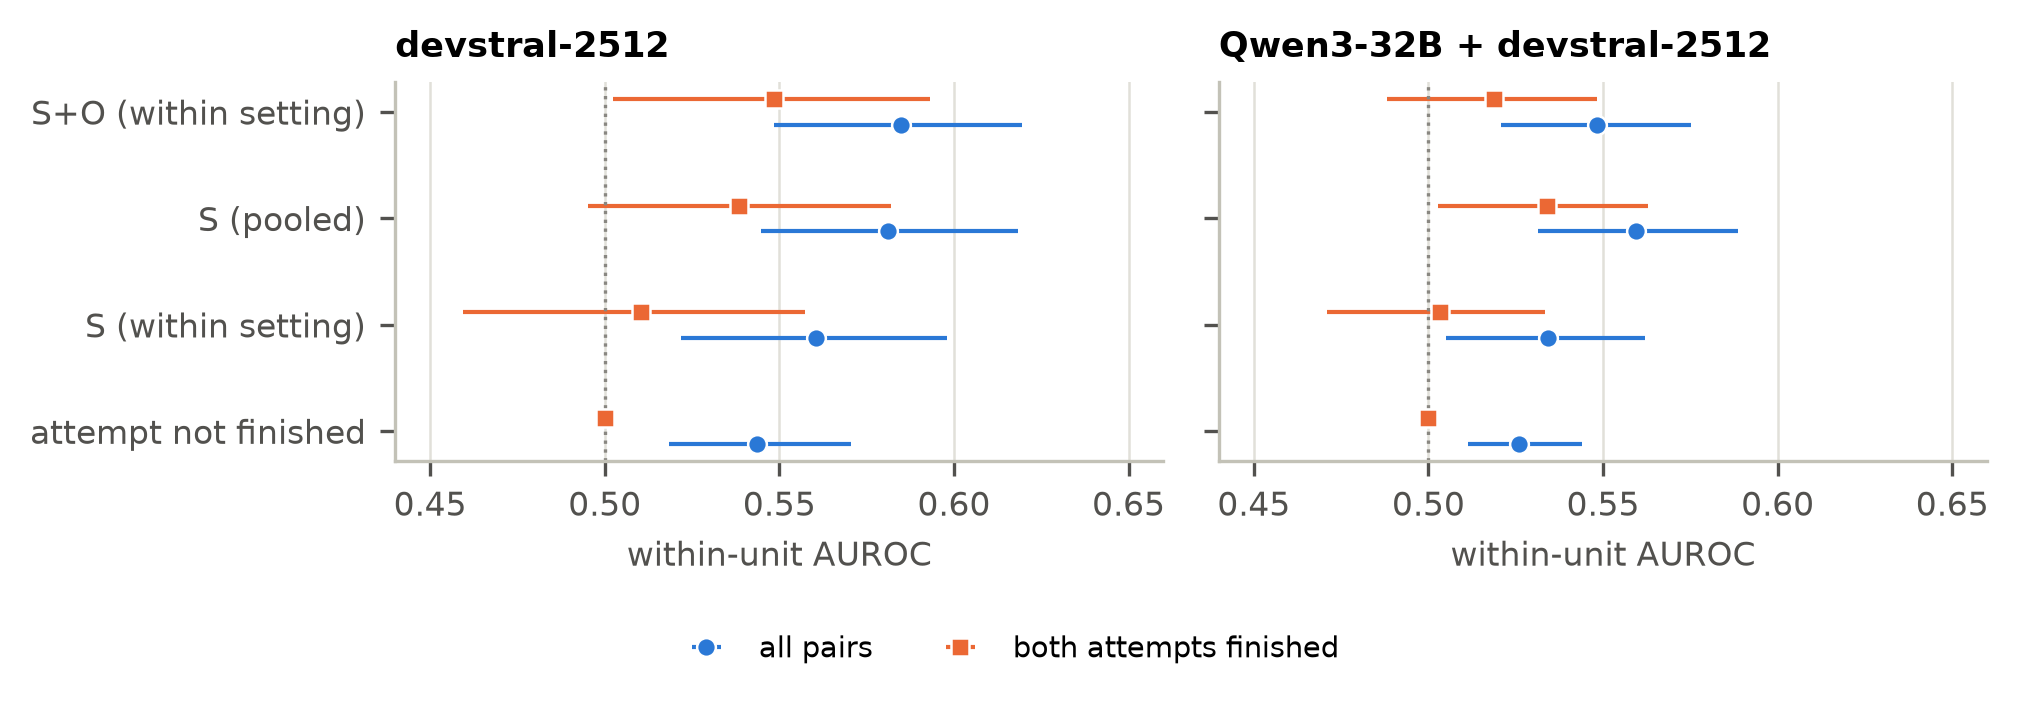
\includegraphics[width=\columnwidth]{fig2_run_level}
\caption{Within-unit AUROC on repeated runs (ASSERT-KTH, two settings). On all pairs the structure model is close to
the single flag `attempt not finished'. Among pairs of finished attempts it is not distinguishable from chance in
either setting (\numsrc{e15k.dev.s2.ff@L120}{0.510 [0.459;\,0.557]} for devstral-2512 with within-setting training);
pooled over both settings it is \numsrc{e15k.both.s1.ff@L128}{0.534 [0.503;\,0.563]} with pooled training and
\numsrc{e15k.both.s2.ff@L130}{0.503 [0.471;\,0.533]} with within-setting training. The agent's own check outcomes
keep a small signal for devstral-2512 (\numsrc{e15k.dev.so2.ff@L123}{0.549 [0.502;\,0.593]} on finished pairs; no
correction for multiple comparisons). Error bars: bootstrap confidence intervals over units.}
\label{fig:run-level}
\end{figure}

\section{The Agent's Words}
\label{sec:words}

% Plan (paper_kit/11_paper_outline.md, part 5; about 0.8 page; claims U12-U14 of 01_thesis_and_claims.md):
% Table III -- spontaneous success claims (detector and after correction), the C4 check on finished pairs, the C3
% check (all pairs and new pairs), differences from S+O and from the claim detector; the distribution of C3 answers
% in one sentence or one table row (Figure 4 is not needed).
% Sources: paper_kit/07_results_agent_words.md; table: paper_kit/10_figures_tables.md (Table III).
\TODO{text of the section on the agent's words and Table III}

\section{Transfer and Limitations}
\label{sec:transfer}

% Plan (paper_kit/11_paper_outline.md, part 6; about 0.5 page; claims U16-U17 of 01_thesis_and_claims.md):
% transfer in one paragraph without a table -- new models of the same log format without loss, a change of format
% with loss; limitations: benchmark saturation, selection of combinations, one model in self-assessment, two settings
% in the repeats, phase rules, multiplicity. Sources: paper_kit/08_transfer_limitations.md.
\TODO{text of the transfer and limitations section}

\section{Related Work}
\label{sec:related}

% Plan (paper_kit/11_paper_outline.md, part 7; about 0.35 page together with the conclusion): 2611.08285 (parallel
% work), 2610.05572, Mehtiyev and Assuncao (an answer to "structure discriminates consistently"), Kaddour et al.,
% Khullar et al., Chen et al., trained verifiers. Keys for the paper: paper_kit/02_related_work.md, section 3.
\TODO{text of the related work section}

\section{Conclusion}
\label{sec:conclusion}

\TODO{text of the conclusion}


\bibliographystyle{IEEEtran}
\bibliography{IEEEtran_control,refs}
\end{document}
